\documentclass{beamer}
\usepackage[utf8]{inputenc}
\usepackage{cite}
\usepackage[english]{babel}
\usepackage{amsmath}
\usepackage{amsthm}
\usepackage{stmaryrd}
\usepackage{minted}
\usepackage{wasysym}
\usepackage{tikz-cd}
\usepackage{adjustbox}
\usepackage{bbold}

\usetikzlibrary{babel}

%\usepackage{reportpage}
\usepackage{amsmath}
\usepackage{bbold}
\usepackage{amssymb}
\usepackage{stmaryrd}
\usepackage{mathrsfs}
\usepackage{scalerel}
\usepackage{multirow}
\usepackage{epsf}
\usepackage{graphics, graphicx}
\usepackage{latexsym}
\usepackage[margin=10pt,font=small,labelfont=bf]{caption}
\usepackage[utf8]{inputenc}
\usepackage[toc,page]{appendix}
\usepackage{subcaption}
\usepackage{tikz}
\usepackage{tikz-cd}
\tikzcdset{scale cd/.style={every label/.append style={scale=#1},
    cells={nodes={scale=#1}}}}
\usepackage{xcolor}
\usetikzlibrary{cd}

\usepackage{amsthm}

\usepackage{lineno}
% \linenumbers

\usepackage{listings}
% basic duo style
\lstdefinestyle{duoStyle}{%
  otherkeywords={case,cocase,def,of,forall,data,codata,rec,mu,import,module,return,set,Top,Bot,CBV,CBN,refinement,constructor,destructor,type,operator,leftassoc,rightassoc,cmd,prd,cns,class,instance,:=,=>,=<,>>,\\\\/,/\\\\,<:,\[,\]},
  morekeywords=[1]{case,cocase,def,of,forall,data,codata,rec,mu,import,module,return,set,Top,Bot,CBV,CBN,refinement,constructor,destructor,type,operator,leftassoc,rightassoc,cmd,prd,cns,class,instance},
  morekeywords=[2]{:=,=>,=<,>>,\\\\/,/\\\\,<:,\[,\]},
  keywordstyle=[1]{\bf\color{blue}},
  keywordstyle=[2]{\bf\color{black}},
  comment=[l]{--},
  commentstyle=\color{gray},
  keywordstyle=\ttfamily\bfseries\color{blue!80!black},
  mathescape=true
  %moredelim=**[is][\bfseries]{|}{|}
}
\lstset{style=duoStyle}


\newenvironment{code}{\captionsetup{type=listing, position=bottom}}{}

% mathbb String
\usepackage{bussproofs}
\EnableBpAbbreviations
\def\ScoreOverhang{0pt}
\def\buildNoScoreTight{% Make an hbox with no score
 \global\setbox\myBoxD=\hbox{\vbox{\vskip0pt}}% 0pt instead of 1pt
}
\def\noLine{% noLine with less space between lines
 \gdef\buildScore{\buildNoScoreTight}%
 \ignorespaces%
}

% noindent on new paragraph
\setlength\parindent{0pt}

% Inference rules
\newcommand{\subPosRule}{\RightLabel{\textsc{Sub}$^+$}}
\newcommand{\subNegRule}{\RightLabel{\textsc{Sub}$^-$}}
\newcommand{\instanceDeclRule}{\RightLabel{\textsc{Decl}}}
\newcommand{\meetRule}{\RightLabel{\textsc{Meet}}}
\newcommand{\joinRule}{\RightLabel{\textsc{Join}}}
\newcommand{\axiomPos}{\RightLabel{\textsc{Axiom}$^+$}}
\newcommand{\axiomNeg}{\RightLabel{\textsc{Axiom}$^-$}}
\newcommand{\topRule}{\RightLabel{\textsc{Top}}}
\newcommand{\botRule}{\RightLabel{\textsc{Bot}}}

\newcommand\deriveRule{
  {\hskip.1in}
  $\stackrel{\mathit{drv}}{\rightsquigarrow}$
  {\hskip.1in}}

\newcommand{\ctx}{\ensuremath{\Gamma \; \vdash \;}}
\newcommand{\opeq}{\ensuremath{\stackrel{op}{\simeq}}}

% Symbols
\newcommand\join{\vee}
\newcommand\meet{\wedge}
\newcommand\sub{\ensuremath{\leqslant}}
\newcommand\transition[1]{\ensuremath{\xrightarrow[]{#1}}}

% Text
\newcommand\Showable{\ensuremath{\Psi_\mathit{Show}}}
\newcommand\Readable{\ensuremath{\Psi_\mathit{Read}}}
\newcommand\Defaultable{\ensuremath{\Psi_\mathit{Default}}}
\newcommand\Ordable{\ensuremath{\Psi_\mathit{Ord}}}
\newcommand\Eq{\ensuremath{\Psi_\mathit{Eq}}}
\newcommand\Monoid{\ensuremath{\Psi_\mathit{Monoid}}}
\newcommand\instance[2]{{\bf instance} \; #1(#2)}
\newcommand\class[2]{{\bf class} \; #1(#2)}

% Terms
\newcommand\caseof[1]{{\bf case}\; #1 \;{\bf of}}
\newcommand\showTerm{{\bf show}}
\newcommand\readTerm{{\bf read}}
\newcommand\ifthenelseTerm{{\bf ifthenelse}\;}
\newcommand\eq{{\bf eq}\;}

% Types
\newcommand\Nat{\mathbb{N}}
\newcommand\Int{\mathbb{Z}}
\newcommand\Unit{\mathbb{U}}
\newcommand\Bool{\mathbb{B}}
\newcommand\Singleton[1]{\mathbb{1}_#1}
\newcommand\String{\mathbb{S}}

% Witnesses
\newcommand\cov{\mathit{cov}}
\newcommand\contrav{\mathit{contrav}}
\newcommand\inv{\mathit{inv}}
% relational composition operator
\newcommand*{\comp}{\mathbin{\raise 0.6ex\hbox{\oalign{\hfil$\scriptscriptstyle
            		 \rm o$\hfil\cr\hfil$\scriptscriptstyle\rm 9$\hfil}}}}
\newcommand\refl{\mathit{refl}}
\newcommand\topW{\mathit{top}}
\newcommand\natPrim{\mathit{natPrim}}
\newcommand\botW{\mathit{bot}}
\newcommand\meetW{\mathit{meet}}
\newcommand\joinW{\mathit{join}}
\newcommand\inW[1]{\mathit{in}_{#1}}
\newcommand\proj[1]{\mathit{proj}_{#1}}
\newcommand\funcW{\mathit{func}}
\newcommand\unfoldL{\mathit{unfold}_{L}}
\newcommand\unfoldR{\mathit{unfold}_{R}}

\newcommand\constraintGen[1]{\ensuremath{\llbracket #1 \rrbracket}}
\newcommand\toConstr{\ensuremath{\hookrightarrow}}
\newcommand\decompose[2]{\ensuremath{{\mathbf{decompose}}(#1 \sub #2)}}

\usepackage{mathpartir}

\setminted{fontsize=\footnotesize}

\title{Type Class Coherence with Subtyping}
\author{Pascal Engel}
\date{June 22 2023}

\setbeamertemplate{navigation symbols}{} % remove annoying buttons
\mode<presentation>

\begin{document}

\begin{frame}
  \centering
  University of T\"ubingen\\
  Department of Computer Science\\
  \maketitle
\end{frame}

\begin{frame}
  \frametitle{Structure}
  \tableofcontents
\end{frame}

\section{Introduction}

\begin{frame}
  \frametitle{Introduction}

  \begin{itemize}
    \item Existing forms of polymorphism to achieve different kinds of program abstraction: Parametricity, subtyping and overloading
    \item New: Combining type classes with subtyping
  \end{itemize}
\end{frame}

\begin{frame}
  \frametitle{Introduction}

  Given $\Phi_{\mathit{Show}}(\{ x : \Nat \})$, do we have an instance for $\Phi_{\mathit{Show}}(\{ x : \Nat, y : \Int \})$?
  \\

  \pause
  Given $\Phi_{\mathit{Read}}(\{ x : \Nat, y : \Int \})$, do we have an instance for  $\Phi_{\mathit{Read}}(\{ x : \Nat \})$?
\end{frame}

\section{Polymorphism}

\begin{frame}
  \frametitle{Polymorphism}

  \begin{itemize}
    \item Parametricity: Theorems for free \cite{wadlertheorems}
    \item Subtyping: Liskov substitution \cite{liskov}
    \item Type classes: Coherent overloading/resolution \cite{reynolds_coherence}
  \end{itemize}
\end{frame}

\section{The Lattice of Types}

\begin{frame}
  \frametitle{The Lattice of Types}

  \begin{prooftree}
    \AxiomC{}
    \RightLabel{\textsc{Refl}}
    \UnaryInfC{$\tau \sub \tau$}
  \end{prooftree}

  % trans
  \begin{prooftree}
    \AxiomC{$\tau \sub \sigma$}
    \AxiomC{$\sigma \sub \rho$}
    \RightLabel{\textsc{Trans}}
    \BinaryInfC{$\tau \sub \rho$}
  \end{prooftree}

  % top/bot
  \begin{center}
    \AxiomC{}
    \RightLabel{\textsc{Top}}
    \UnaryInfC{$\tau \sub \top$}
    \DisplayProof
    {\hskip.2in}
    \AxiomC{}
    \RightLabel{\textsc{Bot}}
    \UnaryInfC{$\bot \sub \tau$}
    \DisplayProof
  \end{center}

  % join intro
  \begin{center}
    \AxiomC{$\tau \sub \sigma$}
    \RightLabel{\textsc{JoinI}$_1$}
    \UnaryInfC{$\tau \sub \sigma \join \rho$}
    \DisplayProof
    {\hskip.2in}
    \AxiomC{$\tau \sub \sigma$}
    \RightLabel{\textsc{JoinI}$_2$}
    \UnaryInfC{$\tau \sub \rho \join \sigma$}
    \DisplayProof
  \end{center}

  \begin{prooftree}
    \AxiomC{$\tau \sub \rho$}
    \AxiomC{$\sigma \sub \rho$}
    \RightLabel{\textsc{JoinI}}
    \BinaryInfC{$\tau \join \sigma \sub \rho$}
  \end{prooftree}

  % meet intro
  \begin{center}
    \AxiomC{$\tau \sub \rho$}
    \RightLabel{\textsc{MeetI}$_1$}
    \UnaryInfC{$\tau \meet \sigma \sub \rho$}
    \DisplayProof
    {\hskip.2in}
    \AxiomC{$\sigma \sub \rho$}
    \RightLabel{\textsc{MeetI}$_2$}
    \UnaryInfC{$\tau \meet \sigma \sub \rho$}
    \DisplayProof
  \end{center}

  \begin{prooftree}
    \AxiomC{$\tau \sub \sigma$}
    \AxiomC{$\tau \sub \rho$}
    \RightLabel{\textsc{MeetI}}
    \BinaryInfC{$\tau \sub \sigma \meet \rho$}
  \end{prooftree}
\end{frame}

\begin{frame}
  \frametitle{The Lattice of Types}
  \begin{prooftree}
    \AxiomC{}
    \RightLabel{\textsc{NatPrim}}
    \UnaryInfC{$\Nat \sub \Int$}
  \end{prooftree}

  \begin{prooftree}
    \AxiomC{$\tau' \sub \tau$}
    \AxiomC{$\sigma \sub \sigma'$}
    \RightLabel{\textsc{Func}}
    \BinaryInfC{$\tau \to \sigma \sub \tau' \to \sigma'$}
  \end{prooftree}

  \begin{prooftree}
    \AxiomC{$\forall j. \tau_j \sub \sigma_j$}
    \AxiomC{$\{ \overline{\ell_j} \} \subseteq \{ \overline{\ell_i} \}$}
    \RightLabel{\textsc{Extend}}
    \BinaryInfC{$\{ \overline{\ell_i : \tau_i} \} \sub \{ \overline{\ell_j : \sigma_j} \}$}
  \end{prooftree}
\end{frame}

\section{Predicates on Types}

\begin{frame}
  \frametitle{Predicates on Types}
  \begin{definition}
    Given a universe of types $\mathcal{U}$, a \emph{predicate over types} $\Phi$ is an element of $\mathcal{P}(\mathcal{U})$.
  \end{definition}

  For our purposes a predicate should additionally be:
  \begin{itemize}
    \item preserved over the subtyping lattice
    \item monotonous, i.e. only depend on the terms of a type
  \end{itemize}
\end{frame}

\begin{frame}
  \frametitle{Predicates on Types}
  
  \begin{prooftree}
    \AxiomC{}
    \RightLabel{\textsc{Axiom}}
    \UnaryInfC{$\Gamma, \Phi(\tau) \vdash \Phi(\tau)$}
  \end{prooftree}

  \begin{prooftree}
    \AxiomC{$\ctx \Phi^<(\sigma)$}
    \AxiomC{$\tau \sub \sigma$}
    \alwaysSingleLine
    \RightLabel{\textsc{CoV}}
    \BinaryInfC{$\ctx \Phi^<(\tau)$}
  \end{prooftree}

  \begin{prooftree}
    \alwaysNoLine
    \AxiomC{$\ctx \Phi^>(\sigma)$}
    \AxiomC{$\sigma \sub \tau$}
    \alwaysSingleLine
    \RightLabel{\textsc{ContraV}}
    \BinaryInfC{$\ctx \Phi^>(\tau)$}
  \end{prooftree}
\end{frame}

\begin{frame}
  \frametitle{Predicates on Types}
  Examples of co-/contravariant type classes (Show, Eq, Ord, Read, Default, ...)\\
  Let $\Gamma := \{ \Showable(\Int), \Defaultable(\Nat) \}$

  \begin{prooftree}
    \AxiomC{}
    \RightLabel{\textsc{Axiom}}
    \UnaryInfC{$\ctx \Showable(\Int)$}
    \RightLabel{\textsc{Prim}$^<$}
    \UnaryInfC{$\ctx \Showable(\Nat)$}
    \RightLabel{\textsc{Meet}$^<_2$}
    \UnaryInfC{$\ctx \Showable(\Singleton{1} \meet \Nat)$}
  \end{prooftree}

  \begin{prooftree}
    \AxiomC{}
    \RightLabel{\textsc{Axiom}}
    \UnaryInfC{$\ctx \Defaultable(\Nat)$}
    \RightLabel{\textsc{Prim}$^>$}
    \UnaryInfC{$\ctx \Defaultable(\Int)$}
    \alwaysSingleLine
    \RightLabel{\textsc{Join}$^>_1$}
    \UnaryInfC{$\ctx \Defaultable(\Int \join \Bool)$}
  \end{prooftree}
\end{frame}

\begin{frame}
  \frametitle{Witnesses}
  We extend the resolution calculus by witness annotations in order to construct evidence that a type satisfies a predicate, i.e. it is an instance of the type class.

  
\end{frame}

\begin{frame}
  \frametitle{Witnesses}
  \begin{prooftree}
    \AxiomC{$w : \instance{\Phi}{\tau}$}
    \RightLabel{\textsc{Decl}}
    \UnaryInfC{$i_\tau(w) : \Phi(\tau)$}
  \end{prooftree}

  \begin{prooftree}
    \alwaysNoLine
    \AxiomC{$w : \Phi^<(\sigma)$}
    \AxiomC{$m : \tau \sub \sigma$}
    \alwaysSingleLine
    \RightLabel{\textsc{CoV}}
    \BinaryInfC{$\cov(w,m) : \Phi^<(\tau)$}
  \end{prooftree}

  \begin{prooftree}
    \alwaysNoLine
    \AxiomC{$w : \Phi^>(\sigma)$}
    \AxiomC{$m : \sigma \sub \tau$}
    \alwaysSingleLine
    \RightLabel{\textsc{ContraV}}
    \BinaryInfC{$\contrav(w,m) : \Phi^>(\tau)$}
  \end{prooftree}
\end{frame}

\begin{frame}
  \frametitle{Witnesses}

  % refl
  \begin{prooftree}
    \AxiomC{}
    \RightLabel{\textsc{Refl}}
    \UnaryInfC{$\refl_\tau : \tau \sub \tau$}
  \end{prooftree}

  % trans
  \begin{prooftree}
    \AxiomC{$f : \tau \sub \sigma$}
    \AxiomC{$g : \sigma \sub \rho$}
    \RightLabel{\textsc{Trans}}
    \BinaryInfC{$f \comp g : \tau \sub \rho$}
  \end{prooftree}

  % top/bot
  \begin{center}
    \AxiomC{}
    \RightLabel{\textsc{Top}}
    \UnaryInfC{$\topW_\tau : \tau \sub \top$}
    \DisplayProof
    {\hskip.2in}
    \AxiomC{}
    \RightLabel{\textsc{Bot}}
    \UnaryInfC{$\botW_\tau : \bot \sub \tau$}
    \DisplayProof
  \end{center}

  % join intro
  \begin{center}
    \AxiomC{$f : \tau \sub \sigma$}
    \RightLabel{\textsc{JoinI}$_1$}
    \UnaryInfC{$\inW{1}(f) : \tau \sub \sigma \join \rho$}
    \DisplayProof
    {\hskip.2in}
    \AxiomC{$f: \tau \sub \sigma$}
    \RightLabel{\textsc{JoinI}$_2$}
    \UnaryInfC{$\inW{2}(f) : \tau \sub \rho \join \sigma$}
    \DisplayProof
  \end{center}

  \begin{prooftree}
    \AxiomC{$f : \tau \sub \rho$}
    \AxiomC{$g : \sigma \sub \rho$}
    \RightLabel{\textsc{JoinI}}
    \BinaryInfC{$\joinW(f,g) : \tau \join \sigma \sub \rho$}
  \end{prooftree}

  % meet intro
  \begin{center}
    \AxiomC{$f : \tau \sub \rho$}
    \RightLabel{\textsc{MeetI}$_1$}
    \UnaryInfC{$\proj{1}(f) : \tau \meet \sigma \sub \rho$}
    \DisplayProof
    {\hskip.2in}
    \AxiomC{$f : \sigma \sub \rho$}
    \RightLabel{\textsc{MeetI}$_2$}
    \UnaryInfC{$\proj{2}(f) : \tau \meet \sigma \sub \rho$}
    \DisplayProof
  \end{center}

  \begin{prooftree}
    \AxiomC{$f : \tau \sub \sigma$}
    \AxiomC{$g : \tau \sub \rho$}
    \RightLabel{\textsc{MeetI}}
    \BinaryInfC{$\meetW(f,g) : \tau \sub \sigma \meet \rho$}
  \end{prooftree}


\end{frame}

\begin{frame}
  \frametitle{Witnesses}

  \begin{prooftree}
    \AxiomC{}
    \RightLabel{\textsc{NatPrim}}
    \UnaryInfC{$\natPrim : \Nat \sub \Int$}
  \end{prooftree}

  \begin{prooftree}
    \AxiomC{$f : \tau' \sub \tau$}
    \AxiomC{$g : \sigma \sub \sigma'$}
    \RightLabel{\textsc{Func}}
    \BinaryInfC{$\funcW(f,g) : \tau \to \sigma \sub \tau' \to \sigma'$}
  \end{prooftree}

  \begin{prooftree}
    \AxiomC{$\forall j. w_j : \tau_j \sub \sigma_j$}
    \AxiomC{$\{ \overline{\ell_j} \} \subseteq \{ \overline{\ell_i} \}$}
    \RightLabel{\textsc{Extend}}
    \BinaryInfC{$\mathit{extend}(\{ w_j \}, \{ \overline{\ell_i} \} \setminus \{ \overline{\ell_j} \}) : \{\overline{\ell_i : \tau_i} \} \sub \{ \overline{\ell_j : \sigma_j} \}$}
  \end{prooftree}


\end{frame}

\section{Type Class Coherence}

\begin{frame}
  \frametitle{Coherence}
  Reynolds \cite{reynolds_coherence}:
  \begin{quote}
    When a programming language has a sufficiently rich type structure, there can be more than one proof of the same
    typing judgment; potentially this can lead to semantic ambiguity since the semantics of a typed language is a function
    of such proofs. When no such ambiguity arises, we say that the language is coherent.
  \end{quote}
\end{frame}

\begin{frame}
  \frametitle{Type Class Coherence}
  Type class resolution decides program semantics
  $\Rightarrow$ To ensure coherence of a program we need to ensure coherence of resolution

  \begin{definition}
    Type class resolution is coherent if and only if for any pair of witnesses $i,j : \Phi(\tau)$ that witness the same predicate application we have $i \opeq j$, i.e. $i$ and $j$ exhibit the same behavior.
  \end{definition}

  Here, it suffices to show that for any pair of witnesses, they contain the same instance declaration.
\end{frame}

\begin{frame}
  \frametitle{Type Class Coherence}

  Covariant predicate: Downwards closed set

  % 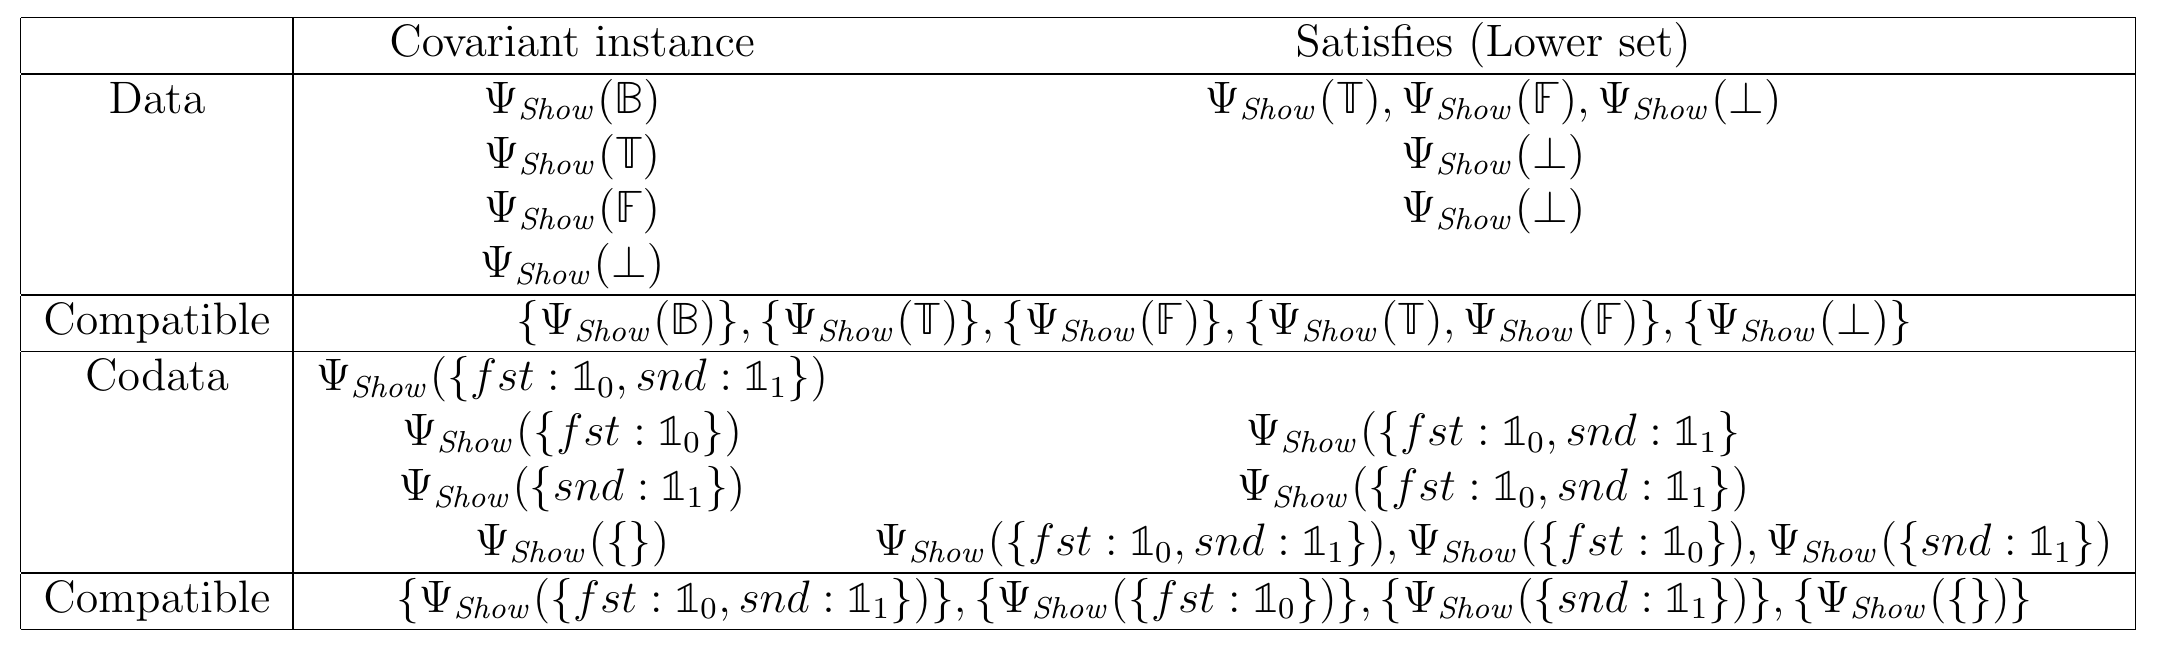
\includegraphics[width=\textwidth]{images/cov_compatible.png}
  % 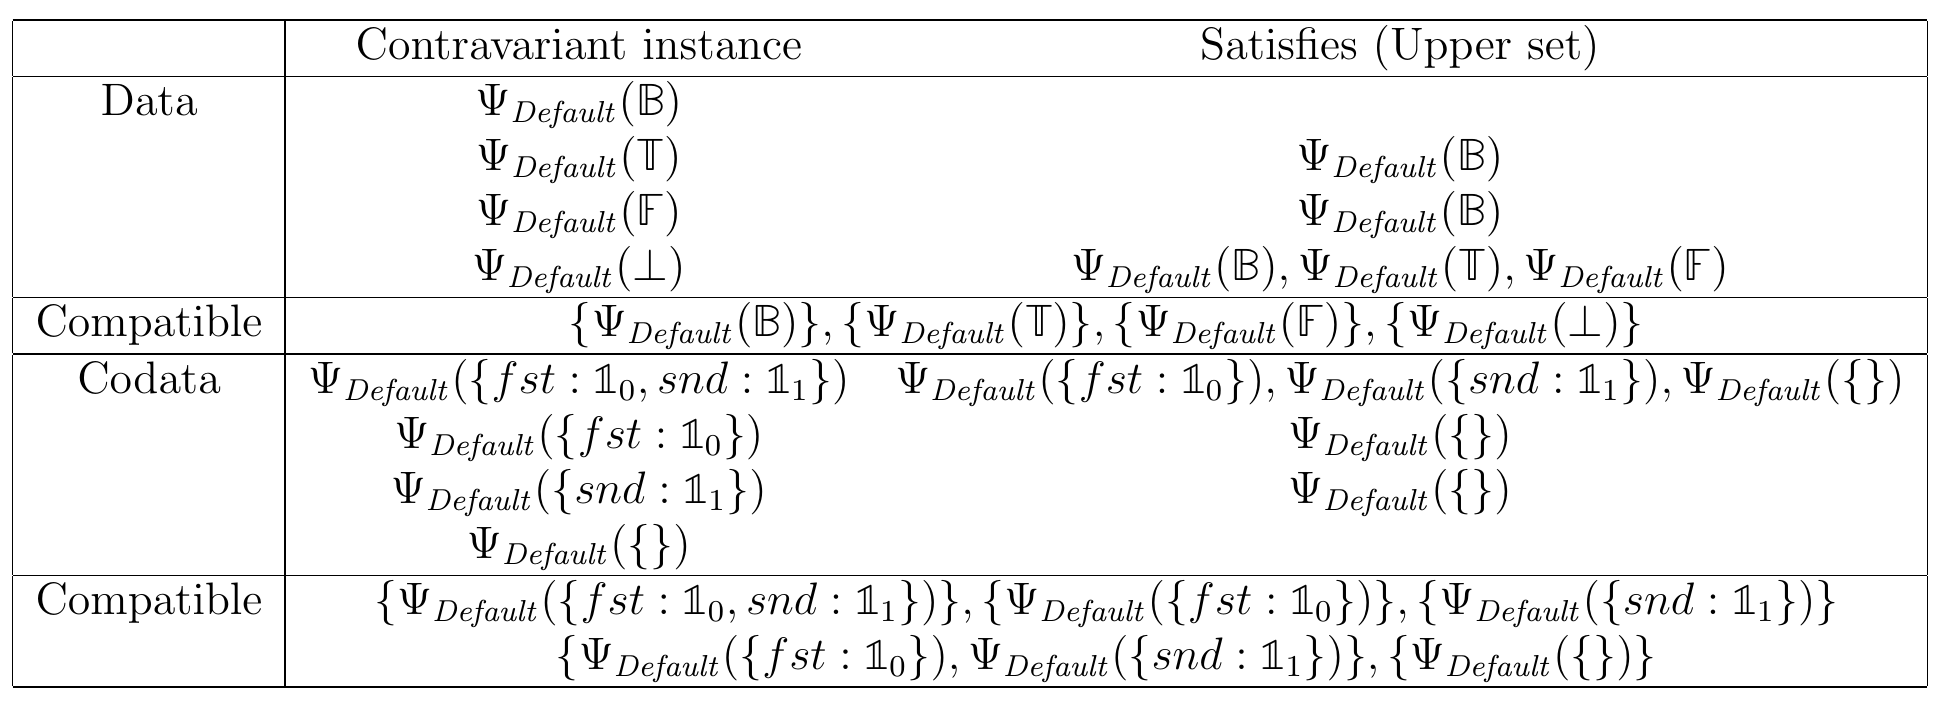
\includegraphics[width=\textwidth]{images/contrav_compatible.png}

  % \[
  % \begin{tikzcd}
  %                                                      & \{ \} \arrow[ld] \arrow[rd]                                  &                                      \\
  %   {\color{blue}\{ fst : \Singleton{0} \}} \arrow[rd] &                                                              & \{ snd : \Singleton{1} \} \arrow[ld] \\
  %                                                      & {\color{blue}\{ fst : \Singleton{0}, snd : \Singleton{1} \}} &
  % \end{tikzcd}
  % \]

  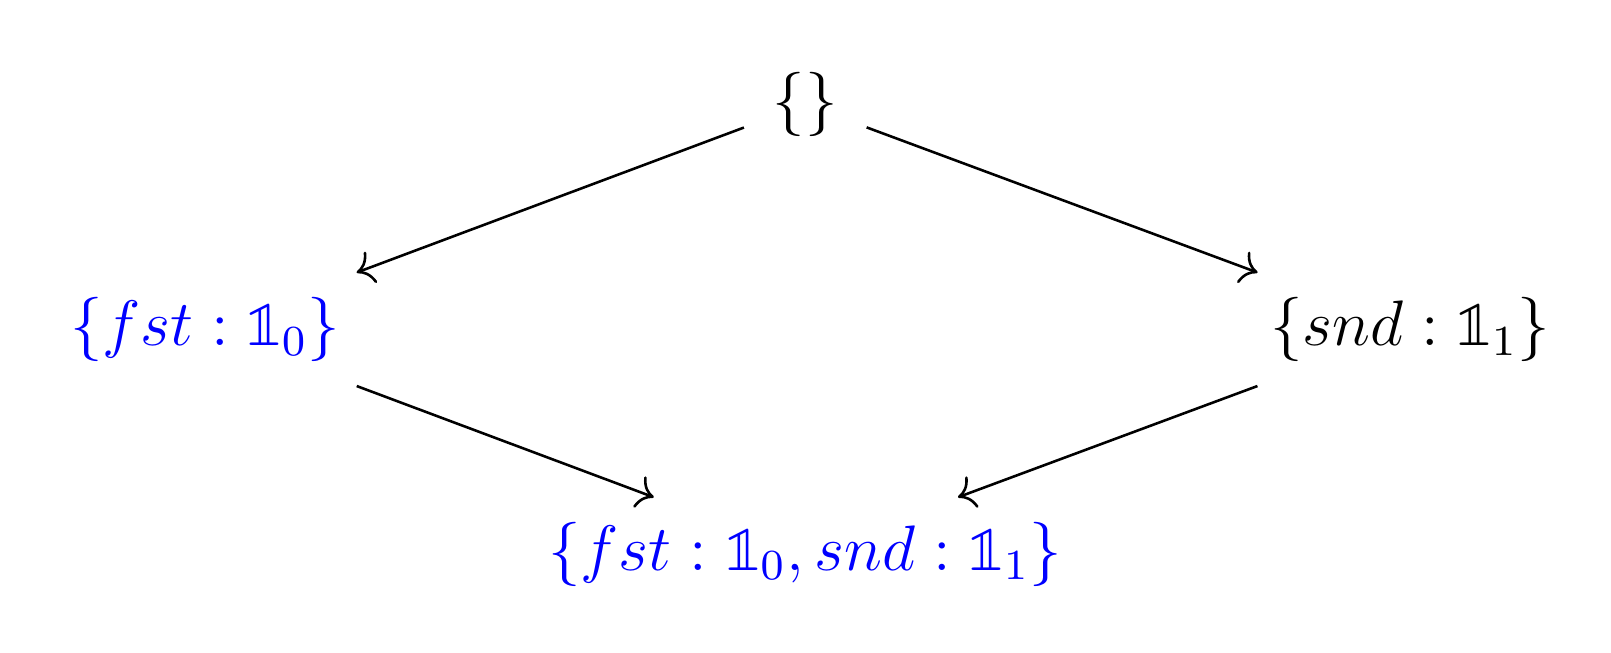
\includegraphics[width=\textwidth]{images/lower_set.png}


\end{frame}

\begin{frame}
  \frametitle{Type Class Coherence}

  Contravariant predicate: Upwards closed set

  % \begin{tikzcd}
  %   &                                                      & {\color{blue}\{\}} \arrow[lld] \arrow[ld] \arrow[d] \arrow[rrd]   &       &                                     \\
  %   \{ \ell_1 : \tau_1 \} \arrow[d] \arrow[rrd]           & {\color{blue}\{ \ell_2 : \tau_2 \}} \arrow[d] \arrow[ld]           & {\color{blue}\{ \ell_3 : \tau_3 \}} \arrow[d] \arrow[ld]          & \dots & \{ \ell_n : \tau_n \} \arrow[llddd] \\
  %   {\{ \ell_1 : \tau_1, \ell_2 : \tau_2 \}} \arrow[rrdd] & {\color{blue}\{ \ell_2 : \tau_2, \ell_3 : \tau_3 \}} \arrow[rdd] & {\{ \ell_1 : \tau_1, \ell_3 : \tau_3 \}} \arrow[dd] & \dots &                                     \\
  %   &                                                      & \dots                                               &       &                                     \\
  %   &                                                      & {\{ \ell_1 : \tau_1, \dots \ell_n : \tau_n \}}      &       &
  % \end{tikzcd}
  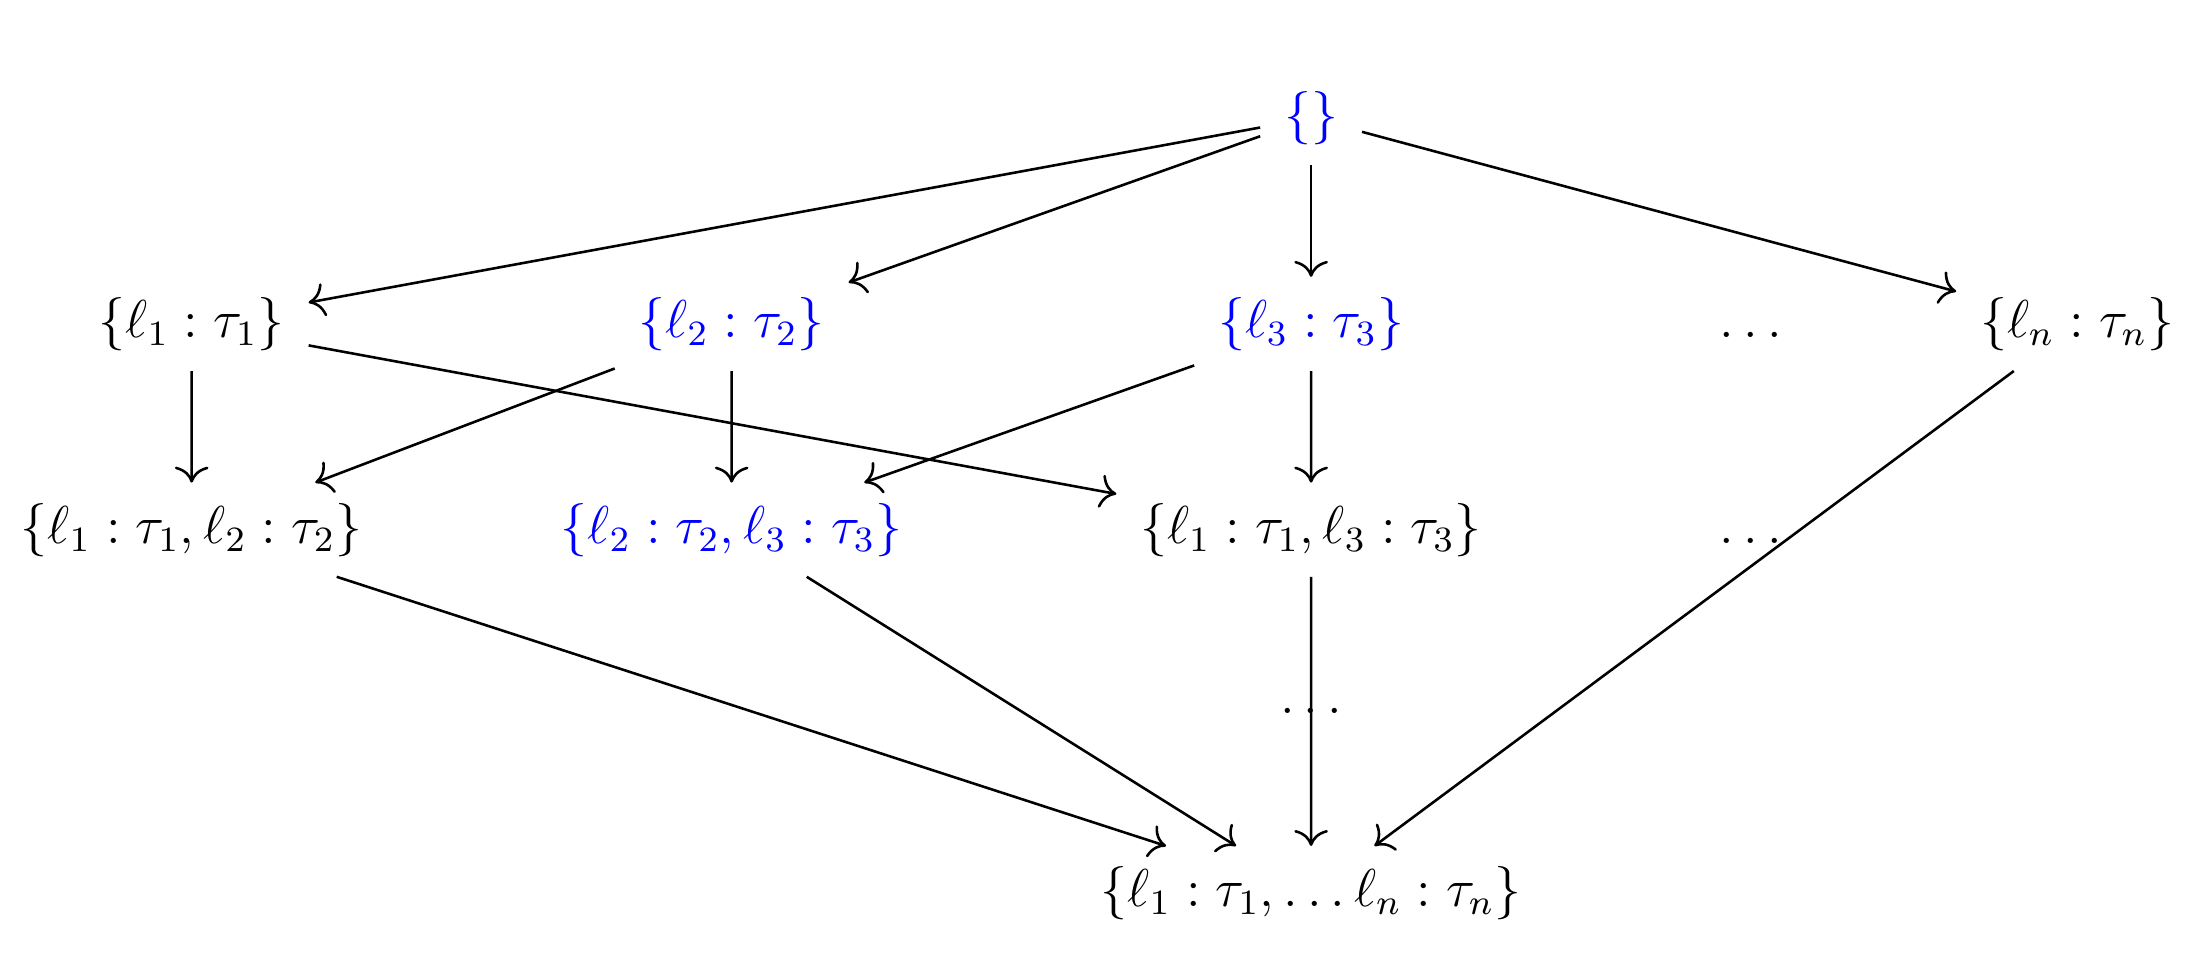
\includegraphics[width=\textwidth]{images/upper_set.png}

  \end{frame}

% \begin{frame}
%   \frametitle{Examples}
% \end{frame}

\begin{frame}
  \frametitle{Summary and Future Work}
  \begin{itemize}
    \item Type classes in a lattice of types are possible
    \item Coherence is even more challenging when resolution is more liberal with co- and contravariant predicates (invariant predicates behave in the usual way)
    \item Further work: Dictionary passing, type schemes with constraints, type inference \& simplification
  \end{itemize}
\end{frame}

\begin{frame}
  \frametitle{Bibliography}
  \footnotesize
  \bibliographystyle{alpha}
  \bibliography{../literature}
\end{frame}

\end{document}